%%%%%%%%%%%%%%%%%%%%%%%%%%%%%%%%%%%%%%%%%%%%%%%%%%%%%%%%%%%%%%%%%%%%%%%%%%%%%%%%
%2345678901234567890123456789012345678901234567890123456789012345678901234567890
%        1         2         3         4         5         6         7         8

\documentclass[letterpaper, 10 pt, conference]{ieeeconf}  % Comment this line out
                                                          % if you need a4paper
%\documentclass[a4paper, 10pt, conference]{ieeeconf}      % Use this line for a4
                                                          % paper

\IEEEoverridecommandlockouts                              % This command is only
                                                          % needed if you want to
                                                          % use the \thanks command
\overrideIEEEmargins
% See the \addtolength command later in the file to balance the column lengths
% on the last page of the document




% The following packages can be found on http:\\www.ctan.org
\usepackage{graphics} % for pdf, bitmapped graphics files
\usepackage{epsfig} % for postscript graphics files
\usepackage{mathptmx} % assumes new font selection scheme installed
\usepackage{times} % assumes new font selection scheme installed
\usepackage{amsmath} % assumes amsmath package installed
\usepackage{amssymb}  % assumes amsmath package installed
\usepackage{hyperref}
\usepackage{units}
\usepackage{ifthen}
\usepackage{tikz}
\usetikzlibrary{calc}
\usepackage[usenames,dvipsnames]{pstricks}
\usepackage{epsfig}
\usepackage{pst-grad} % For gradients
\usepackage{pst-plot} % For axes
\usepackage[space]{grffile} % For spaces in paths
\usepackage{etoolbox} % For spaces in paths
\makeatletter % For spaces in paths
\patchcmd\Gread@eps{\@inputcheck#1 }{\@inputcheck"#1"\relax}{}{}
\makeatother





\title{\LARGE \bf
Recognition of Fingerspelling in Real-time Video Sequence
}

%\author{ \parbox{3 in}{\centering Huibert Kwakernaak*
%         \thanks{*Use the $\backslash$thanks command to put information here}\\
%         Faculty of Electrical Engineering, Mathematics and Computer Science\\
%         University of Twente\\
%         7500 AE Enschede, The Netherlands\\
%         {\tt\small h.kwakernaak@autsubmit.com}}
%         \hspace*{ 0.5 in}
%         \parbox{3 in}{ \centering Pradeep Misra**
%         \thanks{**The footnote marks may be inserted manually}\\
%        Department of Electrical Engineering \\
%         Wright State University\\
%         Dayton, OH 45435, USA\\
%         {\tt\small pmisra@cs.wright.edu}}
%}

\author{Aniket Dhar$^{1}$ and Philipp Duernay$^{2}$% <-this % stops a space
\thanks{$^{1}$Aniket Dhar - 4615808 - a.dhar@student.tudelft.nl}%
\thanks{$^{2}$Philipp Duernay - 4622227 - p.durnay@student.tudelft.nl}%
}




\begin{document}



\maketitle
\thispagestyle{empty}
\pagestyle{empty}


%%%%%%%%%%%%%%%%%%%%%%%%%%%%%%%%%%%%%%%%%%%%%%%%%%%%%%%%%%%%%%%%%%%%%%%%%%%%%%%%
\begin{abstract}

Sign language recognition is a wide field of research where Computer Vision can successfully solve problems for the hearing impaired. We present an application which uses Computer Vision and Machine Learning techniques to recognise fingerspelling sequences from American Sign Language (ASL). The application segments static hand gestures from a video sequence and creates feature descriptors. Those are fed into a trained Support Vector Machine (SVM) classifier for classifying the gestures into letters of the English language. Our system achieves 95\% accuracy in cross-evaluation but fails when applied in the video sequence. We evaluate different approaches for segmentation and feature representation; and present their performance in terms of classification accuracy.  

\end{abstract}


%%%%%%%%%%%%%%%%%%%%%%%%%%%%%%%%%%%%%%%%%%%%%%%%%%%%%%%%%%%%%%%%%%%%%%%%%%%%%%%%
\section{INTRODUCTION}

The accuracy of modern computer vision systems enables a wide range of applications for computers to support society, not only in our daily-life activities, but also in health care or even safety-critical situations. Detection of diseases, cruise control and pedestrian detection are only a few examples to name. 

In this project we explore another possible application for computer vision: the recognition of sign language. As a final goal one can image a smartphone app which translates sign language in real-time, enabling a normal conversation between deaf and hearing people.

As a first step in that direction we start by recognizing the fingerspelling alphabet as shown in \autoref{fig:abc}. We implement and evaluate a computer vision system that can detect the static gestures of this alphabet\footnote{Letter J and Z involve movement and are not part of this project} in a video sequence in real-time. 

\begin{figure}[hb]
\centering
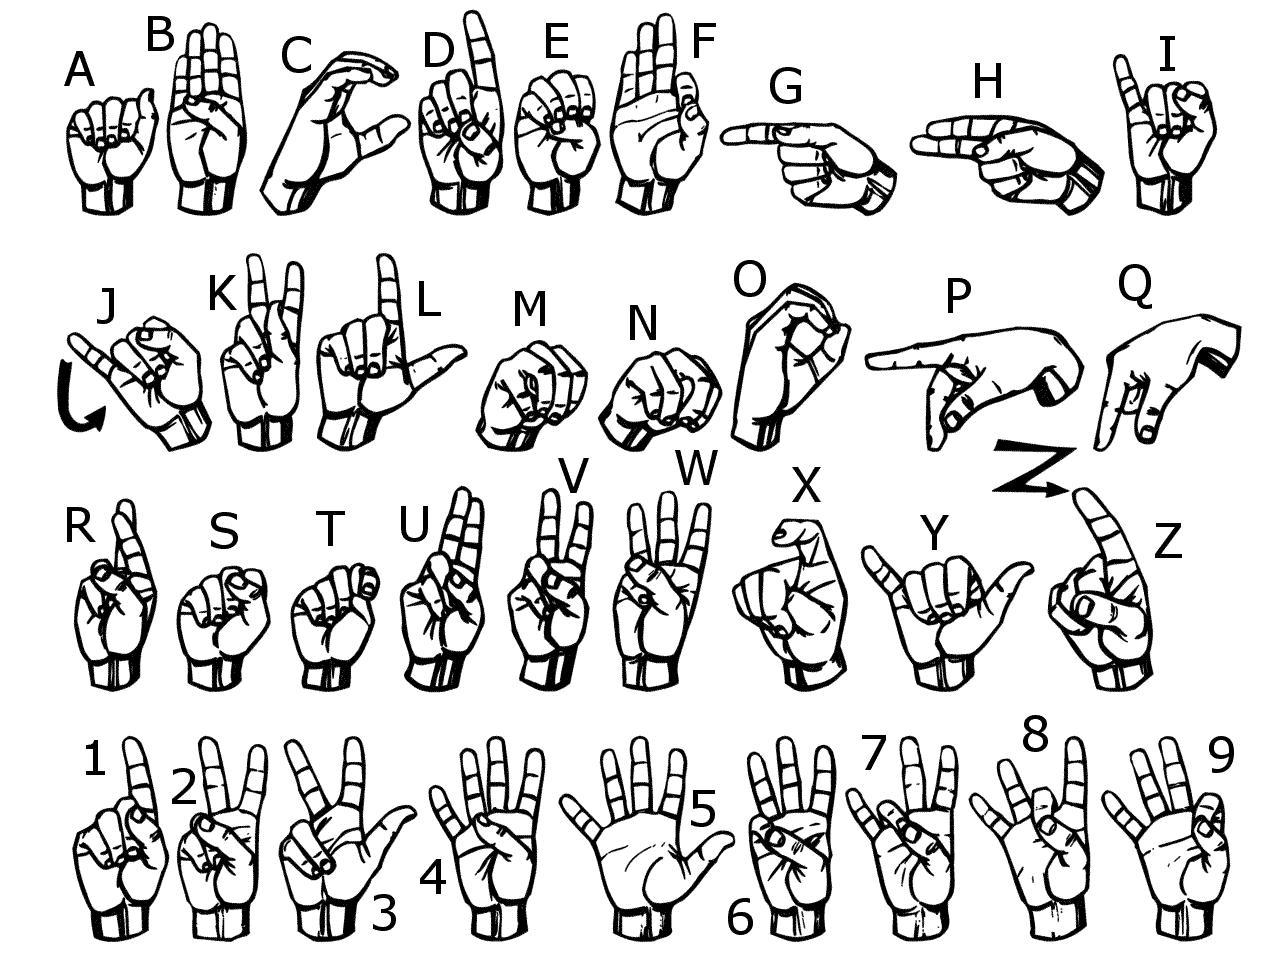
\includegraphics[width=0.8\linewidth]{abc.png}
\caption{American Fingerspelling Alphabet}
\label{fig:abc}
\end{figure}

For that we build a classification system and train it on a dataset of static images. As a proof of concept we embed the obtained model in a small application. The application reads a video stream from the web cam, segments the hand of the user and shows the recognized letter.

For computer vision applications one can make use of a lot of tools and libraries that are already implemented. In this project we use \textit{python3} together with \textit{numpy}, \textit{OpenCV}, \textit{SKlearn} and \textit{PyMaxFlow}. Generally we use \textit{OpenCV} to read images from the web cam and for simple image operations like thresholding, colour space conversion or getting the image gradient. \textit{SKlearn} is used for the classifier implementation and cross-evaluation. \textit{PyMaxFlow} is used for the maxflow/mincut-implementation. A more detailed description of the implementation is given in the respective paragraphs.

The project has been carried out in context of the \textbf{Computer Vision (IN4393)} course at Delft University of Technology. This report describes the work flow of our project, the applied methods as well as the obtained results. The segmentation/representation step turned out to be much harder than originally expected. This is why we mainly focus on this part of the application. Finally, we are able to classify ~95\% of samples correctly on the datasets. However, these results could not be repeated in the web cam application. Here, no letter could be classified correctly.

The remaining parts or this document are structured as follows: \autoref{sec:appr} describes our approach and the implemented methods. \autoref{sec:eval} contains an evaluation of the implemented methods and the respective results. \autoref{sec:concl} concludes the project and gives a short look ahead.


\section{Approach}
\label{sec:appr}
The aim of the project is to recognize letters from the sign alphabet in a video sequence. To achieve this, we take a classical supervised learning approach: we learn a model from labelled examples off-line, then we apply the trained model on video frames.

We identify several parts that are required for the final application: (1) labelled examples on which we can train our model, (2) a segmentation method which separates the hand from the background (2) an object representation that describes the hand unambiguously, (4) a classifier that can train and predict on this representation.

For these steps we tried different approaches. These are described in further detail in the following sections. 

\subsection{Training Data}

We selected two datasets that are suitable for our purpose, namely a set from University of Exeter\footnote{\url{http://empslocal.ex.ac.uk/people/staff/np331/index.php?section=FingerSpellingDataset}} and a set from Thomas Moeslund's\footnote{\url{http://www-prima.inrialpes.fr/FGnet/data/12-MoeslundGesture/database.html}}. For the rest of the document we refer to them as the \textit{ASL-set} and the \textit{TM-set} respectively.

The TM-set contains between 50-100 black and white images per class for the 24 letters of the alphabet. The subjects wear a black sweater and the pictures are taken in front of a black background. An example can be seen in \autoref{fig:tm-set}.

The lightning conditions should make the segmentation quite easy, as there is a big contrast between the hand and the background. However, the lightning conditions are also quite artificial and do not resemble a natural use case. Thus it is questionable whether a model trained on that dataset can perform well in a real application.

The ASL-Set contains 2500 coloured images per class for the 24 letters of the alphabet, taken from 5 different subjects. The pictures have been taken from a kinect camera with more or less equal lightning conditions. An example can be seen in \autoref{fig:asl-set}. Depth data is available for these images, which can be used for segmentation.

The pictures contain strong shadows and a lot of time the face of the user is also visible on the picture. Although this resembles much more our final use case, it makes colour-based segmentation much harder. The depth data can help in segmentation on the dataset, but we can't rely on it in the final use case, as it is not available for our web cam.

\begin{figure}
\centering
\begin{minipage}{0.4\linewidth}
	\centering
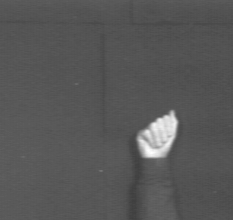
\includegraphics[height=3cm]{a-tm}
\caption{Example image for the TM-set}
\label{fig:tm-set}
\end{minipage}
\hfill
\begin{minipage}{0.4\linewidth}
	\centering
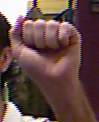
\includegraphics[height=3cm]{a-asl}
\caption{Example image for the ASL-set}
\label{fig:asl-set}
\end{minipage}
\end{figure}


\subsection{Segmentation}

For our project we want to separate the hand from the image background. As the shape of the hand can be different in every image we can't use shape-based features for segmentation. Instead we try several texture-based approaches.

Segmentation can also be seen as a two class classification problem. Given a pixel we are looking for the probability that it belongs to the hand or to the background. Based on that probability we can assign it to one of the two. More formally this would be:

\begin{equation}
	\textbf{assign } y_1 \textbf{ to x if } p(y_1|x) > p(y_0|x) \textbf{ else } y_0
\end{equation}
With $y_1$ as label for the hand and $y_0$ as label for the background. 

\subsubsection{Colour Threshold}

The most straight-forward way is to to use a colour range for segmentation. For example a gray threshold or the skin colour range. As long as the lightning conditions are good and no other objects with the same color are on the image, it can already work reasonably well. 

For this approach we define the likelihood of a pixel being part of the hand:

\begin{equation}
p(y_1 | x) = \begin{cases}
1 & \quad \text{if } \gamma_1 < x < \gamma_2 \\
0 & \quad \text{otherwise}
\end{cases}
\end{equation}
With $\gamma$ as the threshold(s).

This approach can easily be implemented using conditioned indexing with numpy arrays. All pixels of an image that contain a colour value that is higher than a certain threshold are copied to a new image.

We evaluate a gray value threshold on the TM-set, where everything else but the hand is quite dark. An example can be seen in \autoref{fig:tm-cthresh}, where we display the obtained likelihood\footnote{Throughout the document we display the likelihood by scaling it 0-255 and presenting a grayscale image} . 

Here we already get satisfying results. Apart from little noise the hand is clearly visible. 

\begin{figure}[ht!]
\centering
\begin{minipage}{0.4\linewidth}
	\centering
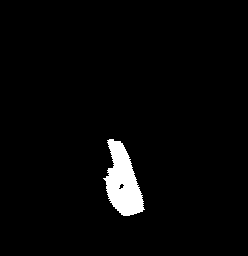
\includegraphics[height=3cm]{tm-segment}
\caption{Colour threshold segmentation on TM-set}
\label{fig:tm-cthresh}
\end{minipage}
\hfill
\begin{minipage}{0.4\linewidth}
	\centering
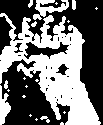
\includegraphics[height=3cm]{asl-segment}
\caption{Colour threshold segmentation on ASL-set}
\label{fig:asl-cthresh}
\end{minipage}
\end{figure}

On the ASL-set we try skin-color-based segmentation. We set a range of (0, 80, 80) to (20, 240, 240) in HSV colour space to be part of the hand and everything else to be background. An example can be seen in \autoref{fig:asl-cthresh}, where we display the obtained likelihood.

One can see that the method does not really work for the ASL-set. Parts from the background, as well as the face of the subject are also segmented.

\subsubsection{Colour Histogram}

A colour histogram consists of a histogram for every colour channel. The histogram can be calculated for a range of pixels and therefore capture a colour distribution over several pixels. Thus it is more reliable than a simple colour threshold.

In our approach we first calculate an average histogram for hand pixels, then we define the class conditional probability as the difference to that average histogram. Inspired by the last lab session we define the likelihood as:

\begin{equation}
p(y_1 | x) = e^{-\frac{d(\bar{\phi},\phi(x))}{\sigma}}
\label{eq:hist}
\end{equation}
Where $\phi$ denotes the histogram function, \textbf{d} denotes the KL divergence and $\sigma$ is a scaling factor.

Also this approach can be implemented with \textit{numpy} arrays. The calculation of the KL divergence we integrate from the \textit{MATLAB} script of the last lab session to python.

On the ASL-set the hand is in almost all cases in the center of the picture. Thus we can obtain the average histogram taking the average histogram for a 6-by-6 window in the center of the picture across the whole dataset. Then we can apply \autoref{eq:hist} with a 6-by-6 sliding window over every image. An example can be seen in \autoref{fig:asl-hist-segment}, where the likelihood is displayed.

\begin{figure}
		\centering
		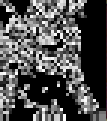
\includegraphics[height=3cm]{asl-hist-segment}
		\caption{Likelihood of the colour histogram method}
		\label{fig:asl-hist-segment}
\end{figure}
One can easily see that the results are not satisfactory. Although big parts of the background are separated properly, the method fails on image parts where the colour is similar to skin colour. This can be seen at the face of the subject, as well as the yellow background. Another problem is the big differences even on the hand. All together we don't consider this approach as promising enough.

\subsubsection{Background Subtraction}

Background subtraction is a way to separate fore- and background in videos. A background frame is calculated and subtracted from the current frame. Thus only objects that changed their appearance remain in the distance image.

As our application will only run on a stationary web cam, we can assume that the hand is the only moving object and background subtraction is applicable. However, the approach can't be applied during training, where we only have static images available.

For the calculation of the background frame we take an average across several frames. We define a likelihood model for background subtraction as follows:

\begin{equation}
p(y_1 | x) = e^{-\frac{|\bar{x}-x|)}{\sigma}}
\label{eq:backg}
\end{equation}
Where $\bar{x}$ is the background, and $\sigma$ a scaling factor.

We implement this using \textit{OpenCV}. After some blurring, we use \texttt{accumulatedSum()} to calculate the average image and \texttt{absdiff()} to subtract the background.

An example for a described distance image can be seen in \autoref{fig:bg-subtr}. The method looks promising as the hand is clearly separable. However, if we move the hand slowly, or the lightning conditions are bad, big parts of the hand are also taken as background.

\begin{figure}[ht!]
\centering
	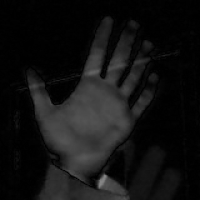
\includegraphics[height=3cm]{bg-subtr}
	\label{fig:bg-subtr}
	\caption{Distance image for background subtraction}
\end{figure}

\subsubsection{Depth Segmentation}

For the ASL-set depth data is available. An example can be seen in \autoref{fig:asl-depth}, where the depth data for \autoref{fig:asl-set} is displayed as gray scale image. The low resolution of the data is apparent as only about 5 different levels are visible.

To use the depth data for segmentation, we measure the depth at the center of the image and take it as baseline. Then we calculate the likelihood as follows:

\begin{equation}
p(y_1 | x) = e^{-\frac{|x_{center}-x|)}{\sigma}}
\label{eq:backg}
\end{equation}
Where $x_ {center}$ is depth value at the center of the image, and $\sigma$ a scaling factor.

Also here the implementation is quite straight forward. The image is stored in a similar way as a grayscale image. Thus we can subtract the depth value of the center from the whole image and obtain the distance matrix.

An example of the obtained likelihood can be seen in Fig. ref{fig:depth-segment}. Although depth segmentation enables us to separate the background partly, for most pictures it is not enough to segment the hand entirely. However, we can use the method in combination with other segmentation methods.

\begin{figure}[ht!]
	\centering
	\begin{minipage}{0.4\linewidth}
		\centering
		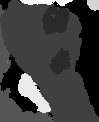
\includegraphics[height=3cm]{asl-depth}
		\caption{Depth data int the ASL-set}
		\label{fig:asl-depth}
	\end{minipage}
	\hfill
\begin{minipage}{0.4\linewidth}
\centering
	
\includegraphics[height=3cm]{depth-segment}
	\label{fig:depth-segment}
	\caption{Likelihood for depth segmentation}
	\end{minipage}
\end{figure}

\begin{figure}
\end{figure}


\subsubsection{Nearest Neighbour Classifier}

Instead of just measuring values on the image we can also train a classifier on labelled examples. As we want to do the segmentation for the video in real-time, we need a classifier that can be trained quickly. This makes the kNN-classifier a good choice.

Labelled examples are unfortunately not available in the given data set, so we use a hands-on method to obtain those. Similar to the histogram method we sample a window of 6-by-6 pixels in the picture center as objects with label $y_1$. Additionally we can use depth segmentation or background subtraction to obtain background samples with label $y_0$. 

Once the classifier is trained it can be used to label the whole image. As we did not implement the classifier ourselves we don't go into detail about its functionality here and refer to standard pattern recognition literature.

For the implementation we use the 3-nearest-neighbour implementation from \textit{sklearn}. The library allows training a model and obtaining predictions.

\begin{figure}
\centering
	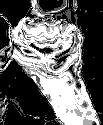
\includegraphics[height=3cm]{knn-segment}
	\label{fig:knn-segment}
	\caption{Soft labels of k-NN classifier}
\end{figure}

An example can be seen in \autoref{fig:knn-segment}, where the likelihood is displayed. We see that most parts of the hand are separated quite nicely. However, the method fails whenever there are strong shadows on the hand. As the colour is way different compared to other parts of the hand, the classifier assigns a low likelihood. One can also see that parts that have a similar colour to the hand get a higher soft label e.g. the ear of the subject.

\subsubsection{Markov Random Field}

A Markov Random Field (MRF) enables the incorporation of spatial conditions with label probabilities. We use it to combine these spatial conditions with several of the methods described before.

We apply the depth segmentation and background subtraction model to get soft labels for back and foreground. Additionally we train the knn-classifier as described and obtain another set of soft labels for the image. Then we can define the combined likelihood as a weighted sum of the score of the nearest neighbour classifier and of the background calculation. This can be formulated as follows:
\begin{equation}
p(y_1 | x) = \alpha * s_{knn}(y_1 | x) + \beta * s_{backgr}(y_1 | x) 
\end{equation}
With $\alpha$ and $\beta$ as weights and $s_{knn}$ and $s_backgr$ as the respective soft labels.

This way we incorporate colour information and background/foreground information in our likelihood model. Ideally this compensates the individual weaknesses of both methods, such as strong colour changes for the kNN-classifier or inaccuracy of the background calculation.

An example for the combined likelihood can be seen in \autoref{fig:comb-segment}. Although only slightly, one can see an improvement compared to the individual labellings.

We tune $\alpha$ and $\beta$ on a visual basis on several random images. This way we choose $\alpha = 0.6$ and $\beta=0.4$.
\begin{figure}
\centering
	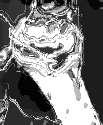
\includegraphics[height=3cm]{comb-segment}
	\label{fig:comb-segment}
	\caption{Combined Likelihood}
\end{figure}

For defining spatial structures we take the image gradient. We want the edge value of the MRF to drop when there was an edge in the initial image. Therefore we assign edges on y and x axis with the respective gradients $I_y, I_x$ multiplied by -1.

In total this gives us the following Markov Random Field:
\begin{center}

\psscalebox{0.8 0.7} % Change this value to rescale the drawing.
{
\begin{pspicture}(0,-4.2)(5.285984,4.2)
\label{fig:mrf-graph}
\psellipse[linecolor=black, linewidth=0.04, dimen=outer](2.6,3.6)(0.6,0.6)
\psellipse[linecolor=black, linewidth=0.04, dimen=outer](0.6,0.04)(0.6,0.6)
\psellipse[linecolor=black, linewidth=0.04, dimen=outer](4.6921678,0.06)(0.5938165,0.58)
\psellipse[linecolor=black, linewidth=0.04, dimen=outer](2.7,-3.64)(0.58,0.56)
\psellipse[linecolor=black, linewidth=0.04, dimen=outer](2.64,0.12)(0.6,0.6)
\psellipse[linecolor=black, linewidth=0.04, dimen=outer](3.82,1.24)(0.58,0.56)
\psellipse[linecolor=black, linewidth=0.04, dimen=outer](1.54,-1.08)(0.6,0.6)
\psline[linecolor=black, linewidth=0.04, arrowsize=0.05291667cm 2.0,arrowlength=1.4,arrowinset=0.0]{<-}(0.82689905,0.7149105)(2.24,3.16)
\psline[linecolor=black, linewidth=0.04](1.1875665,0.023503793)(2.0924335,0.056496207)
\psline[linecolor=black, linewidth=0.04](3.0637367,0.4422136)(3.7362633,1.1177864)
\psline[linecolor=black, linewidth=0.04](3.2675664,0.023503793)(4.1724334,0.056496207)
\psline[linecolor=black, linewidth=0.04](1.9037366,-0.6777864)(2.5762634,-0.0022135878)
\psline[linecolor=black, linewidth=0.04, arrowsize=0.05291667cm 2.0,arrowlength=1.4,arrowinset=0.0]{<-}(2.6,0.76)(2.56,3.04)
\psline[linecolor=black, linewidth=0.04, arrowsize=0.05291667cm 2.0,arrowlength=1.4,arrowinset=0.0]{<-}(1.626899,-0.44508946)(2.36,3.04)
\psline[linecolor=black, linewidth=0.04, arrowsize=0.05291667cm 2.0,arrowlength=1.4,arrowinset=0.0]{<-}(3.52,1.72)(2.88,3.04)
\psline[linecolor=black, linewidth=0.04, arrowsize=0.05291667cm 2.0,arrowlength=1.4,arrowinset=0.0]{<-}(4.48,0.8)(3.040533,3.1537228)
\psline[linecolor=black, linewidth=0.04](0.72,-0.64)(0.92,-0.96)
\psline[linecolor=black, linewidth=0.04, arrowsize=0.05291667cm 2.0,arrowlength=1.4,arrowinset=0.0]{->}(1.8270663,-1.6564572)(2.48,-3.16)
\psline[linecolor=black, linewidth=0.04, arrowsize=0.05291667cm 2.0,arrowlength=1.4,arrowinset=0.0]{->}(2.6596117,-0.5451615)(2.68,-3.04)
\psline[linecolor=black, linewidth=0.04, arrowsize=0.05291667cm 2.0,arrowlength=1.4,arrowinset=0.0]{->}(4.3823037,-0.5819679)(3.08,-3.12)
\psline[linecolor=black, linewidth=0.04, arrowsize=0.05291667cm 2.0,arrowlength=1.4,arrowinset=0.0]{->}(3.6670663,0.62354285)(2.88,-3.08)
\psline[linecolor=black, linewidth=0.04, arrowsize=0.05291667cm 2.0,arrowlength=1.4,arrowinset=0.0]{->}(1.44,-1.76)(2.28,-3.28)
\rput[bl](3.44,2.64){$p(y_1|x)$}
\rput[bl](3.68,-2.4){$p(y_0|x)$}
\rput[bl](2.48,3.44){$y_1$}
\rput[bl](2.6,-3.8){$y_0$}
\rput[bl](4.56,-0.04){$x_2$}
\rput[bl](1.4,-1.2){$x_3$}
\rput[bl](0.48,-0.08){$x_0$}
\rput[bl](2.56,0.0){$x_1$}
\rput[bl](3.72,1.12){$x_4$}
\rput[bl](3.6,-0.28){$-I_x$}
\rput[bl](2.04,-0.84){$-I_y$}
\rput[bl](1.16,0.2){$-I_x$}
\rput[bl](2.72,0.64){$-I_y$}
\end{pspicture}
}


\end{center}

Now we only need to cut the graph where the weights are minimal. This can be done using the maxflow graph cut algorithm.

For the implementation we use the \texttt{maxflow} package for python. The package allows us to define a graph and to assign weights according to \autoref{fig:mrf-graph}. Subsequently we can execute the maxflow algorithm and obtain the labeled image. The first result still contains some noise. Therefore we apply several bluring/eroding and closing operations of OpenCV, to obtain a cleaner result.

An example for the method can be seen in \autoref{fig:mrf-example} and \autoref{fig:mrf-example-video}, where we display the images after segmentation. The results look quite promising and in this first evaluation we consider it as our best method so far.

\begin{figure}
	\centering
	\begin{minipage}{0.4\linewidth}
		\centering
		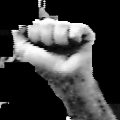
\includegraphics[height=3cm]{mrf}
		\label{fig:mrf-example}
		\caption{Segmentation with Markov Random Field on ASL-set}
	\end{minipage}
	\hfill
	\begin{minipage}{0.4\linewidth}
		\centering
		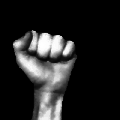
\includegraphics[height=3cm]{mrf-video}
		\label{fig:mrf-example-video}
		\caption{Video Segmentation with Markov Random Field}
	\end{minipage}
\end{figure}


\subsection{Representation}

Once the hand is properly segmented from the background we need to define descriptors for the hand shape that enable an accurate recognition. As we are interested in the shape of the hand, shape based descriptors seem to be a reasonable approach at first. However, also these need to be obtained from the image. In several letters it is particular necessary to also capture the shape of the fingers inside the hand and not only the overall shape. In the ASL-set and on the video there are a lot of shadows in the pictures which make this not an easy task.

Therefore we mainly work with region-based descriptors. The approaches are described in the following.

\subsubsection{Grayscale-Pixel}

This can be seen as one of the most straight-forward representation. We convert the segmented image to a grayscale image, vectorize it and obtain the feature vector.

The drawback of the method is that less important features are not particularly filtered, which results in a huge feature vector. These are generally harder to classify (Curse of dimensionality). Additionally, the representation is not rotation/scale invariant.

\subsubsection{Histogram of Gradients}

HoG-features \cite{c1} are commonly used for object detection. The image gradient is calculated for the whole image. Then for a fixed window size a histogram of the gradient directions is formed.

These features incorporate direction of change in intensity value and should therefore be more informative than the simple Gray-Pixel representation. However, the same drawback as described in the previous paragraph holds. The representation is not rotation/scale invariant.

For our application we use a 6-by-6 window on a 60-by-60 image and 16 bins. In contrast to the first method we need our own implementation for HoG-features. We use OpenCV to obtain the image gradients, subsequently we calculate the angular and magnitude using numpy functions.

\subsubsection{Bag of HoGs}

To compensate for the rotation invariance we apply a "Bag-of-" method. Here we apply a KMeans clustering to obtain the most common histograms of the ASL-dataset as a codebook. Then we represent each object by the distance to this codebook. Inspired by MILES \cite{c2} calculate the distance as follows:

\begin{equation}
	\phi(x) = \max\limits_j\quad e^{\frac{-||x_j-x_{codebook}||^2}{\sigma}}
\end{equation}

Thus the distance of an image to a code word is defined by the distance of its closest instance. The measure should give a high similarity if the HoGs of two objects are similar even if they are at different places in the image.

This method basically builds upon the previous method. After having obtained the HoG-features for all images, we use KMeans clustering from the \textit{sklearn} library to get the codebook.

\subsubsection{Principal Component Analysis}

A general way to deal with high dimensionality or less informative features is principal component analysis. Here we transform the feature space by keeping the maximal variance. We use PCA on top of the previously described methods. The principal components are chosen in a way that 90\% of the variance is kept.

Even here we use the \textit{sklearn} library as it provides functions to scale the data, as well as to apply PCA.

\subsection{Classification}

After having segmented the image and transformed it to a representation we can train a classifier. The focus of the work was on the preceeding steps, which is why we only evaluate one classifier and compare the different representations.

We use a linear Support Vector Machine for classification as it generally performs well and can deal with high dimensionality. The implementation has been taken from the \textit{sklearn} library.

In the video the user will not change the shown letter every couple of milliseconds. Thus we have several frames per sample available and can exploit that for classification. 

We take a sequence of 5 frames per sample and classify each. The final prediction is based on a majority vote. Additionally we can set a "confidence" threshold to avoid misclassification. If at least 75 \% of the predictions are not same, we reject the classification and "Letter not recognized" message is displayed on the screen.

The majority voting was implement ourselves. The classifiers are taken from \textit{sklearn} library.

\section{Evaluation}
\label{sec:eval}
We select several combinations among the most promising methods described in the previous chapters for final evaluation. As a first step, we evaluate the methods on the two datasets in cross-evaluation. The methods with the best results are trained on the whole dataset and evaluated in the video.

For all of the methods exist several parameters, such as the number of neighbours for the kNN-classifier, the weights for the weighted sum or the number of bins in the histogram, that can also influence performance. These should be fine tuned to obtain best possible results. However, the set of parameters is large and a full evaluation would be beyond the scope of this project. 

\subsection{Performance on Datasets}

We set up a 6-folded cross-evaluation for all methods where we measure the mean performance in accuracy and its standard derivation. An overview of the evaluated methods and their results is given in \autoref{tab:eval-methods}

\begin{table}[h]
\caption{Evaluated methods}
\label{tab:eval-methods}
\begin{center}
\begin{tabular}{c|c|c|c|c}
Dataset & Segmentation & Representation & Classifier & Accuracy \\
\hline
\hline
TM-set & Gray-thresh & Gray-Pixel & SVM & 0.71($\pm$ 0.032)\\
TM-set & Gray-thresh & HoG & SVM & 0.94($\pm$ 0.035)\\
ASL-set & MRF & Gray-Pixel & SVM & 0.73($\pm$ 0.004)\\ 
ASL-set & MRF & HoG & SVM & 0.96($\pm$ 0.001)\\
ASL-set & MRF & Bag of HoGs & SVM & 0.083 $\pm$ 0.001\\
\hline
\end{tabular}
\end{center}
\end{table}

The improvement on the HoG features representation is significant. In both cases the results improved by about 20\%. This is somewhat expected as the HoG features in contrast to the Gray-thresh representation, capture changes across several pixels. These seem to be distinctive for the hand gestures.

With the Bag-of-Hogs representation we tried to find a more rotation/translation invariant descriptor and thus achieve better discriminabilty . However, it seems our approach had the opposite effect. As we define the distance of a bag by its closest instance, we basically allow the HoGs to be everywhere and completely loose the order. It seems that the overall distribution of HoGs in images of the dataset is somewhat equal, which leads we assume to the low performance of the approach.

In contrast to our original expectations, we achieve better results on the ASL-set. This is despite the fact that those pictures are way harder to segment than the pictures of the TM-set. However, we also have much more training data here. The amount of samples could compensate for the harder segmentation.

We also assume that the Markov-Random-Field segmentation paid off and contributed to the good results on the ASL-set. Earlier experiments with simpler segmentation methods had a way lower performance.

The best results we obtained on the ASL-set with MRF-segmentation and HoG-features. As this dataset also resembles much more our use case, we select this model to be applied in the video.

\subsection{Performance on Video}

For the video evaluation we show every letter once (for 5 frames) and record the prediction given by the classification system. Unfortunately, our implementation does not work much better than random guessing. In none of the test cases the letter could be classified correctly.

A reason for this could be the fact that the conditions on the dataset and in the video are still too different. For example we did try to avoid having disturbing objects in the video frame, to get better segmentation results in the video. For the dataset segmentation in contrast this was not possible so we had to train the model on more noisy data. This could have led to a model that is overfitted to the imperfect segmentation on the dataset, achieves good results there but fails in the real application.


\section{CONCLUSIONS}
\label{sec:concl}

Initially, we defined three main parts for our application. For each of these we tried different approaches. We conclude this report by describing the respective outcomes.

We found two datasets from which we considered one very suitable for our application, as it resembled our use case. However, the segmentation on this dataset was not an easy task. Thus we could not really get the same representation from the dataset as we got from the video frames. We assume we would have better results, if we would have labelled examples that look similar to the ones we get from the video segmentation. In a future work we could create our own dataset and revalidate our methods.

Generally the segmentation step turned out to be harder than initially expected. After trying several approaches that did not lead to satisfying results, we came up with a Markov Random Field approach to exploit as much information as possible. This led to decent up to good results on the dataset and on the video frames. The results could probably be even better if a dataset with annotated pixels is used. Then we would not have to rely on our hands-on method to obtain samples and other classifiers could be tried for segmentation. Unfortunately we could not find such a dataset.

Next to the simple approach of using gray values directly, we tried a HoG- and a Bag-of-Hogs approach for representation. Although the first two methods are not scale/rotation invariant, they achieved much better results than the Bag-of-Hogs approach. Here, too much spatial information was lost for good classification. We conclude that HoG is well-working approach for hand-gesture recognition.

All in all, we are satisfied with the progress we made throughout the project despite the bad performance on the video. In our initial experiments, we achieved classification results lower than 10\%. Subsequently, we applied several concepts learnt during class and improved the classification results to 95\%. Hence, this work served as a good step towards a fingerspelling recognition application.

\addtolength{\textheight}{-12cm}   % This command serves to balance the column lengths
                                  % on the last page of the document manually. It shortens
                                  % the textheight of the last page by a suitable amount.
                                  % This command does not take effect until the next page
                                  % so it should come on the page before the last. Make
                                  % sure that you do not shorten the textheight too much.

%%%%%%%%%%%%%%%%%%%%%%%%%%%%%%%%%%%%%%%%%%%%%%%%%%%%%%%%%%%%%%%%%%%%%%%%%%%%%%%%



%%%%%%%%%%%%%%%%%%%%%%%%%%%%%%%%%%%%%%%%%%%%%%%%%%%%%%%%%%%%%%%%%%%%%%%%%%%%%%%%
\begin{thebibliography}{99}

\bibitem{c1} Dalal, Triggs. (2005). Histograms of oriented gradients for human detection, CVPR 2005. IEEE Computer Society Conference, San Diego, USA, 25 June . IEEE.

\bibitem{c2}Chen, Yixin and Bi, Jinbo and Wang, James Ze,(2006).MILES: Multiple-instance learning via embedded instance selection,IEEE Transactions on Pattern Analysis and Machine Intelligence,vol.28-12,1931-1947.IEEE.



\end{thebibliography}


%%%%%%%%%%%%%%%%%%%%%%%%%%%%%%%%%%%%%%%%%%%%%%%%%%%%%%%%%%%%%%%%%%%%%%%%%%%%%%%%





\end{document}
